
\documentclass[11pt,a4paper,sans]{moderncv} 

\moderncvstyle{casual}    
\moderncvcolor{green} 

\usepackage[utf8]{inputenc}
\usepackage[russian]{babel}
\usepackage{hyperref}
\hypersetup{
    colorlinks=true,
    linkcolor=blue,
    filecolor=magenta,      
    urlcolor=blue
}


\setlength{\hintscolumnwidth}{2cm}

% adjust the page margins
\usepackage[scale=0.8]{geometry}

% personal data
\name{}{Глеб Пушкарев}
\title{Резюме \\ +7(952)666-13-10 \\ gleb.pushkarev@gmail.com \\
Github: \href{https://github.com/NelosG}{NelosG}}
\phone[mobile]{+7(952)666-13-10}                  
\email{gleb.pushkarev@gmail.com}
\social[github]{NelosG}                            

\makeatletter\renewcommand*{\bibliographyitemlabel}{\@biblabel{\arabic{enumiv}}}\makeatother

\begin{document}
\makecvtitle

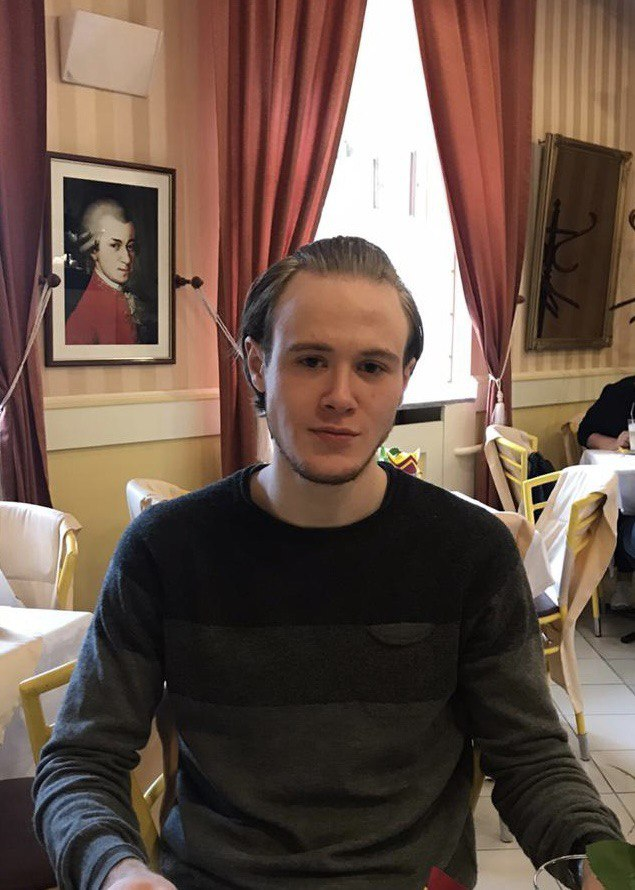
\includegraphics[width=0.35\columnwidth]{photo.jpg}\\[\baselineskip]
\section{Профессия, специальность}
\cvitem{}{Kotlin/Java разработчик}

\section{Высшее образование}
\cvitem{2019-2024}{Университет ИТМО,}
\cvitem{}{Кафедра Компьютерных Технологий,} 
\cvitem{}{Специальность Прикладная математика и информатика}

\section{Опыт Работы}
\cvitem{2020-2020}{Стажировка в ООО\grqqМРГТ\grqq(Системный администратор)}
\cvitem{2022-2022}{\href{https://github.com/NelosG/softwerke-internship}{Практика} в ООО\grqqСофтверке\grqq(Java1.8 + OSGi)}   
\cvitem{2022}{Младший разработчик ООО\grqqСолантек\grqq}
\cvitem{}{}
\cvitem{}{}
\cvitem{}{}

\section{Ключевые навыки}
\cvitem{Осн.}{Kotlin, Java, Spring, Maven, PostgreSQL, Liquibase}
\cvitem{Доп.}{C++, CMake, Git, Shell, OSGi, Haskell}


\section{Знание Языков}
\cvitem{Русский}{Родной}
\cvitem{Английский}{B1+}

\section{Учебные проекты}
\cvitem{Github}{\href{https://github.com/NelosG/ITMO-KT}{ITMO KT}}


 \section{Пройденные курсы}
\cvitem{}{Алгоритмы и структуры данных, Дискретная математика,}
\cvitem{}{Математический анализ, Линейная алгебра, Дифференциальные уравнения,}
\cvitem{}{Программирование на Java, Advanced Java, Курс C++, Advanced C++,}
\cvitem{}{Теория вероятности, Математическая статистика,}
\cvitem{}{Архитектура ЭВМ, Операционные системы,}
\cvitem{}{Телекоммуникационные системы и технологии, Методы трансляции,}
\cvitem{}{Методы оптимизации, Математическая логика, Параллельное программирование,}
\cvitem{}{Анализ данных, Машинное обучение, Рекомендательные системы,}
\cvitem{}{Фронтенд, Функциональное программирование (Haskell)}

\end{document}
